%set the master document for easy compilation
%!TEX root = ../D3_5_3.tex

\section{F2.3: trainData}

\subsection{Component Requirements}

\begin{longtable}{p{.25\textwidth}p{.7\textwidth}}
\toprule
Component name			& trainData \\
\midrule
Link to SCADE model		& {\footnotesize \url{https://github.com/openETCS/modeling/blob/master/model/Scade/System/ObuFunctions/manageData/trainData/trainData.etp}} \\
\midrule
SCADE designer			& Bernd Hekele, DB Netz AG \\
\midrule
Description				& Implementation of the train data with the corresponding interfaces to track, driver and RBC.

This component provides the storage of train data and the procedures necessary for updating data and controlling interfaces for validating train data at the DMI and to the RBC. 

The scope of train data is defined in section 3.18.3 of the SRS. Train data are qualifying some safety relevant properties of the train like the length of the train, maximal speed and brake behaviour. 

During startup of the EVC a first definition of the train data is received from the train interface unit (TIU). During Start of Mission the data is updated resp. validated by the driver via action on the Driver Machine Interface (DMI).  The driver may change some of the data. He has to confirm the set of data before being able to push the start button.
 
When setting up a radio session to an RBC the evc has to send the actual train data to the RBC for vaildation:
Message Flow:
\begin{itemize}
\item sending Message 129 (Validated Train Data)
\item receiving Message 8 (Acknowledment of Train Data) is processed as apart of the validation procedure with the RBC.
\item sending Message 146 (Acknolwedement) in the context of this message flow. T\_TRAIN parameter of the messages is used to confirm the association of the messages.
\end{itemize}

The trainData component uses a dedicated state for controlling the reception of the acknowledgement.\\
\midrule
Input documents	& Subset-026, Chapter 3.18.3\\
\midrule
Safety integrity level	& 4 \\
\midrule
Time constraints		& n/a \\
\midrule
API requirements 		& Train Data needs systemtime for stamping messages, access to input from the track messages and access to the output of RBC messages.\\
\bottomrule
\end{longtable}


\subsection{Interface}

An overview of the interface of component trainData is shown in Figure~\ref{f:traindata_interface}. The inputs and outputs are described in detail in Section~\ref{s:traindata_inputs} respectively \ref{s:traindata_outputs}. Subcomponents are described in Section~\ref{s:traindata_subcomponents}.

\begin{figure}
\center
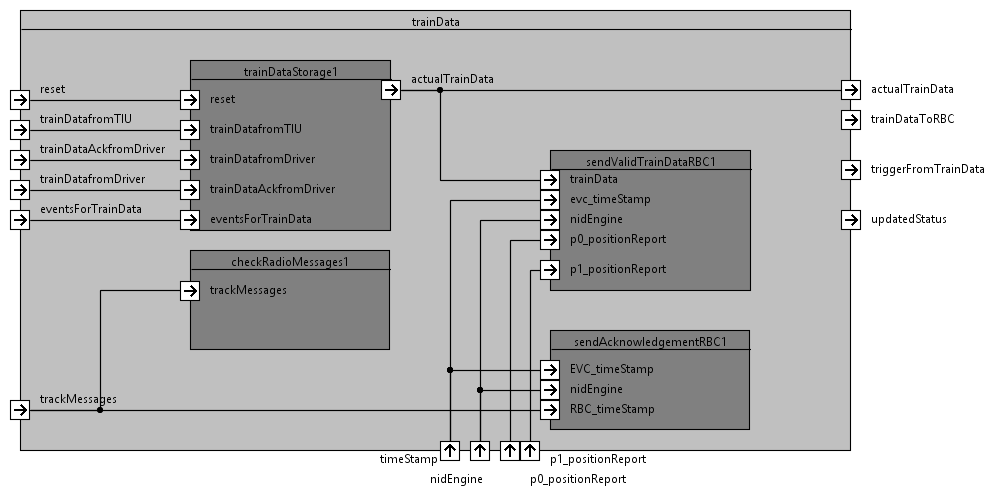
\includegraphics[width=\textwidth]{./images/Figure_15_IBD_manageTrainData_1.png}
\caption{trainData component SysML diagram}\label{f:traindata_interface}
\end{figure}


\subsubsection{Inputs}\label{s:traindata_inputs}

\paragraph{reset}

\begin{longtable}{p{.25\textwidth}p{.7\textwidth}}
\toprule
Input name				& reset \\
\midrule
Description				& Triggers the reset of the train data and the train data status data.\\
\midrule
Source					& Persistant data status management.\\ 
\midrule
Type					& bool \\
\midrule
Valid range of values	& 
\begin{description}
\item[true] Perform reset of train data and train data status.
\item[false] No reset of data in this cycle.
\end{description}
\\
\midrule
Behaviour when value is at boundary	& n/a \\
\midrule
Behaviour for values out of valid range	& n/a \\
\midrule
Behaviour when value is erroneous, absent or unwanted (i.e. spurious) & n/a \\
\bottomrule
\end{longtable}

\paragraph{trainDatafromTIU}

\begin{longtable}{p{.25\textwidth}p{.7\textwidth}}
\toprule
Input name				& trainDatafromTIU \\
\midrule
Description				& Train data received via TIU. The availability of data is indicated with the valid flag. This data is expected to be received in the first place. In the current implementation it is not supported to change data after a mission has been started.  The structure covers the following compontents:
\begin{description}
\item[valid](bool): valid indicator for this component. In this structure valid means the data has been received from train. Addition states like validated by driver or validated by RBC are maintained in the status structure for train data.
\item[other components]:  Other components are defined according to section 3.18.3.2 of subset 26. 
\end{description} \\
\midrule
Source					& Train Interface Unit (TIU) \\ 
\midrule
Type					& TIU\_Types\_Pkg::trainData\_T \\
\midrule
Valid range of values	& Input with valid information is indicated with the valid flag. 
\\
\midrule
Behaviour when value is at boundary	& n/a\\
\midrule
Behaviour for values out of valid range	& When valid flag indicates false the data to be used is assumed to be default values. The component is not used when valid flag is false.\\
\midrule
Behaviour when value is erroneous, absent or unwanted (i.e. spurious) & Information is only expected at Start of Mission Procedure. Once the information is successfully received it is not considered any more. Change of train data by train during mission is not supported by this version of the openETCS OBU model.\\
\bottomrule
\end{longtable}

\paragraph{trainDatafromDriver}

\begin{longtable}{p{.25\textwidth}p{.7\textwidth}}
\toprule
Input name				& trainDatafromDriver \\
\midrule
Description				& Train data received via DMI from the driver. The availability of data is indicated with the valid flag. The data is expected as a mandatory parameter during start of mission. In the current implementation it is not supported to change data after a mission has been started. The structure consists of the following components:
\begin{description}
\item[valid](bool): valid indicator for this component. The data has been received from DMI. The flag is set to TRUE for a single cycle. 
\item[systemTime](Obu\_BasicTypes\_Pkg::T\_internal\_Type): timestamp set by the DMI. The component is not used by trainData.
\item[trainCtategory](NC\_TRAIN): Train category used for the static speed profile calculation.
Thanks to NC\_TRAIN, the train knows the SSP it must obey. Each bit represents one category. A train can belong to various categories.
\item[l\_train](Obu\_BasicTypes\_Pkg::L\_internal\_Type): Length of the train [cm].
\item[m\_brakeperct](int): brake percentage. range from 0 to 300.
\item[v\_maxtrain](Obu\_BasicTypes\_Pkg::V\_internal\_Type): maximum speed of the train in km/h.
\todo[inline]{needs to be changed to cm/sec}
\item[m\_axleLoad](M\_AXLELOADCAT): axle load category according to 3.18.3.2
\item[m\_airTight](M\_AIRTIGHT): airtight system presence according to 3.18.3.2
\item[m\_loadingGauge](M\_LOADINGGAUGE): loading gauge category according to 3.18.3.2
\end{description} \\

\midrule
Source					& Driver Machine Interface (DMI) \\ 
\midrule
Type					& DMI\_Messages\_Bothways\_Pkg::DMI\_Train\_Data\_T \\
\midrule
Valid range of values	& Input with valid information is indicated with the valid flag. \\
\midrule
Behaviour when value is at boundary	& n/a\\
\midrule
Behaviour for values out of valid range	& When valid flag indicates false the data to be used is assumed to be default values. The component is not used when valid flag is false.\\
\midrule
Behaviour when value is erroneous, absent or unwanted (i.e. spurious) & No checks on individual values is done in this part of the openETCS EVC. We assume - if necessary - appropriate checks are part of the interface layer (e.g., CRC checks) This type of checks is not in the scope of the openETCS project.\\
\bottomrule

\end{longtable}

\paragraph{trainDataAckfromDriver}

\begin{longtable}{p{.25\textwidth}p{.7\textwidth}}
\toprule
Input name				& trainDataAckfromDriver \\
\midrule
Description				& During start of mission the driver has to validate the train data. The confirmation is visible  based on this input. The structure looks like:
\begin{description}
\item[valid](bool): valid indicator for this component. The data has been received from DMI. The flag is set to TRUE for a single cycle. 
\item[systemTime](Obu\_BasicTypes\_Pkg::T\_internal\_Type): timestamp set by the DMI. The component is not used by trainData.
\item[acknowledged](bool): Result of the driver's acknoledgment.
\end{description} \\
\\
\midrule
Source					& Driver Machine Interface (DMI) \\ 
\midrule
Type					& DMI\_Messages\_DMI\_to\_EVC\_Pkg::DMI\_Train\_Data\_Ack\_T \\
\midrule
Valid range of values	& Input with valid information is indicated with the valid flag. In addition, the ack parameter has to be evaluated in order to recognise the decision of the driver.\\
\midrule
Behaviour when value is at boundary	& n/a\\
\midrule
Behaviour for values out of valid range	& when valid flag indicates false the data to be used is assumed to be default values. The component is not used when valid flag is false.\\
\midrule
Behaviour when value is erroneous, absent or unwanted (i.e. spurious) & no checking on individual values is done in this part of the openETCS EVC. We assume - if necessary - appropriate checks are part of the interface layer (e.g., CRC checks) This type of checks is not in the scope of the openETCS project.\\

\bottomrule
\end{longtable}
\paragraph{trackMessages}

\begin{longtable}{p{.25\textwidth}p{.7\textwidth}}
\toprule
Input name				& trackMessages \\
\midrule
Description				& Information carries the message received from RBC. Information is only used when the valid flag is true and the message source is Radio. Other information is not relevant. Information is evaluated as long as the validation procedure is not completed and a valdiation request with the RBC is pending. \\
\midrule
Source					& Radio Transmission Module (RTM)\\ 
\midrule
Type					& Common\_Types\_Pkg::ReceivedMessage\_T \\
\midrule
Valid range of values	& Input with valid information is indicated with the valid flag.\\
\midrule
Behaviour when value is at boundary	& n/a\\
\midrule
Behaviour for values out of valid range	& 
When valid flag indicates false the data to be used is assumed to be default values. The component is not used when valid flag is false.\\
\midrule
Behaviour when value is erroneous, absent or unwanted (i.e. spurious) & 
No checking on individual values is done in this part of the openETCS EVC. We assume - if necessary - appropriate checks are part of the interface layer (e.g., CRC checks) This type of checks is not in the scope of the openETCS project.\\

\bottomrule
\end{longtable}

\paragraph{timeStamp}

\begin{longtable}{p{.25\textwidth}p{.7\textwidth}}
\toprule
Input name				& timeStamp \\
\midrule
Description				& Timestamp for messaging to the RBC.\\
\midrule
Source					& Derived from train time.\\ 
\midrule
Type					& T\_TRAIN\\
\midrule
Valid range of values	& Positive non-zero real\\
\midrule
Behaviour when value is at boundary	& Parameter is not used for computation or addressing. No impact in this model.\\
\midrule
Behaviour for values out of valid range	& No impact in the EVC. Communication to the RBC will be broken.\\
\midrule
Behaviour when value is erroneous, absent or unwanted (i.e. spurious) & Communication to the RBC will be broken. No safety issue in the EVC since RBC connection errors are covered by the EVC function.
\\
\bottomrule
\end{longtable}


\paragraph{eventsForTrainData}

\begin{longtable}{p{.25\textwidth}p{.7\textwidth}}
\toprule
Input name				& eventsForTrainData\\
\midrule
Description				& Timestamp for messaging to the RBC. Information of the EVC relevant for train data handling according to Section 3.18.3. In the current state of implementation the following events are evaluated:
\begin{itemize}
\item train stand-still
\item communication Session established
\end{itemize}
The MoRC ready input is used to indicate the evc:morc function is ready with acknowledgment of the communication session.\\
\midrule
Source					& EVC model.\\ 
\midrule
Type					& trainData\_Types\_pkg::trainData\_Events\_T\\
\midrule
Valid range of values	& Structure of a set of bool. Each component may be true or false.\\
\midrule
Behaviour when value is at boundary	& n/a\\
\midrule
Behaviour for values out of valid range	& n/a\\
\midrule
Behaviour when value is erroneous, absent or unwanted (i.e. spurious) & n/a\\

\bottomrule
\end{longtable}

\paragraph{nidEngine}

\begin{longtable}{p{.25\textwidth}p{.7\textwidth}}
\toprule
Input name				& nidEngine\\
\midrule
Description				& Id of the engine. This id is used in communication with the RBC in order to uniquely identify the engine.\\
\midrule
Source					& Configuration\\ 
\midrule
Type					& NID\_ENGINE\\
\midrule
Valid range of values	& Structure of a set of bool. Each component may be true or false.\\
\midrule
Behaviour when value is at boundary	& n/a\\
\midrule
Behaviour for values out of valid range	& n/a\\
\midrule
Behaviour when value is erroneous, absent or unwanted (i.e. spurious) & n/a\\

\bottomrule
\end{longtable}
\paragraph{p0\_positionReport}

\begin{longtable}{p{.25\textwidth}p{.7\textwidth}}
\toprule
Input name				& p0\_positionReport\\
\midrule
Description				& Actual Position Report (packet 0) for communication with the RBC.
\\
\midrule
Source					& EVC model.\\ 
\midrule
Type					& Packet\_TrainTypes\_Pkg::PT0\_PositionReport\_T\\
\midrule
Valid range of values	& This packet is administered by a valid flag.\\
\midrule
Behaviour when value is at boundary	& n/a\\
\midrule
Behaviour for values out of valid range	& n/a\\
\midrule
Behaviour when value is erroneous, absent or unwanted (i.e. spurious) & n/a\\

\bottomrule
\end{longtable}

\paragraph{p1\_positionReport}

\begin{longtable}{p{.25\textwidth}p{.7\textwidth}}
\toprule
Input name				& p1\_positionReport\\
\midrule
Description				& Actual Position Report (packet 1) for communication with the RBC.
\\
\midrule
Source					& EVC model.\\ 
\midrule
Type					& Packet\_TrainTypes\_Pkg::PT1\_PositionReport\_2BG\_T\\
\midrule
Valid range of values	& This packet is administered by a valid flag.\\
\midrule
Behaviour when value is at boundary	& n/a\\
\midrule
Behaviour for values out of valid range	& n/a\\
\midrule
Behaviour when value is erroneous, absent or unwanted (i.e. spurious) & n/a\\

\bottomrule
\end{longtable}

\subsubsection{Outputs}\label{s:traindata_outputs}

\paragraph{actualTrainData}

\begin{longtable}{p{.25\textwidth}p{.7\textwidth}}
\toprule
Output name				& actualTrainData \\
\midrule
Description				& Actual train data of the evc. Train data received via DMI from the driver. The availability of data is indicated with the valid flag. The data is expected as a mandatory parameter during start of mission. In the current implementation it is not supported to change data after a mission has been started. The structure consists of the following components:
\begin{description}
\item[valid](bool): valid indicator for this component. Valid indicates the data are updated after start-up of the system. The actual status of trainData is stored in the updatedStatus information. 
\item[acknowledgedByDriver](bool): Indicates this component has been validated by the driver.
\todo[inline]{redundant information to status. Needs cleaning}
\item[trainCtategory](NC\_TRAIN): Train category used for the static speed profile calculation.
\item[cantDeficientcy](NC\_CDTRAIN): Cant deficiency train category
\item[trainLength](Obu\_BasicTypes\_Pkg::L\_internal\_Type): Length of the train [cm].
\item[brakePercentage](int): brake percentage. range from 0 to 300.
\item[maxTrainSpeed](Obu\_BasicTypes\_Pkg::V\_internal\_Type): maximum speed of the train in km/h.
\todo[inline]{needs to be changed to cm/sec}
\item[loadingGauge](M\_LOADINGGAUGE): loading gauge category according to 3.18.3.2
\item[axleLoadCategory](M\_AXLELOADCAT): axle load category according to 3.18.3.2
\item[airTightSystem](M\_AIRTIGHT): airtight system presence according to 3.18.3.2
\item[axleNumber]int): axle number according to 3.18.3.2
\item[numberNationalSystems](int): The number of national systems available in the train.
\item[nationalSystems](Packet\_TrainTypes\_Pkg::aNID\_NTC\_T): National Systems available in the train. The elements 0 .. numberNationalSystems - 1 are carrying the relevant data.
\item[numberTractionSystems](int): The number of traction systems available in the train.
\item[tractionSystems](Packet\_TrainTypes\_Pkg::aTractionIdentity\_T): Traction Systems available in the train. The elements 0 .. numberTractionSystems - 1 are carrying the relevant data.
\end{description} \\


\midrule
Destination				& evc \\ 
\midrule
Type					& TIU\_Types\_Pkg::trainData\_T \\
\midrule
Valid range of values	& n/a \\
\midrule
Behaviour when value is at boundary	& n/a \\
\midrule
Behaviour for values out of valid range	& n/a \\
\midrule
Behaviour when value is erroneous, absent or unwanted (i.e. spurious) &n/a \\
\bottomrule
\end{longtable}

\paragraph{trainDataToRBC}

\begin{longtable}{p{.25\textwidth}p{.7\textwidth}}
\toprule
Output name				& trainDataToRBC \\
\midrule
Description				& Messages for communicating with the RBC. Messages 129 (Validated Train Data) and 146 (Acknowledgement) are sent by this function. The presence of the message is indicated by a valid flag.\\
\midrule
Destination				& Radio Output \\ 
\midrule
Type					& Radio\_Types\_Pkg::Radio\_TrainTrack\_Message\_T \\
\midrule
Valid range of values	& indicated by valid flag. \\
\midrule
Behaviour when value is at boundary	& n/a\\
\midrule
Behaviour for values out of valid range	& n/a \\
\midrule
Behaviour when value is erroneous, absent or unwanted (i.e. spurious) & n/a\\
\bottomrule
\end{longtable}

\paragraph{triggerFromTrainData}

\begin{longtable}{p{.25\textwidth}p{.7\textwidth}}
\toprule
Output name				& triggerFromTrainData \\
\midrule
Description				& For a full implementation of ETCS trainDAta has additional tasks described in the standard but not implemented in openETCS. For those extensions the triggers are pre-defined. \\
\midrule
Destination				& evc \\ 
\midrule
Type					& trainData\_Types\_pkg::trainData\_Trigger\_T
 \\
\midrule
Valid range of values	& n/a \\
\midrule
Behaviour when value is at boundary	& n/a\\
\midrule
Behaviour for values out of valid range	& n/a \\
\midrule
Behaviour when value is erroneous, absent or unwanted (i.e. spurious) & n/a\\
\bottomrule
\end{longtable}

\paragraph{updatedStatus}

\begin{longtable}{p{.25\textwidth}p{.7\textwidth}}
\toprule
Output name				& updatedStatus \\
\midrule
Description				& Detailed definition of the trainData status. The following components are defined:
\begin{description}
\item[valid](bool): Data is initialised based on data received from the TIU.
\item[validatedByDriver](bool): Data has been validated by the Driver.
\item[validatedbyRBC](bool): Data has been validated by the RBC.
\item[waitingForRBCResponse](bool): 3.18.3.4.1 Train is waiting for ack to validation command.
\item[driverIsModificationTrainData](bool):3.18.3.3.1 Driver is Modifying / Revalidating train data.
\item[timeStampValidateToRBC](T\_TRAIN): 8.7.4 This label is used in communication with the RBC to identify the communication entity. Train data is acknowledged.
\end{description} 
\\
\midrule
Destination				& evc \\ 
\midrule
Type					& trainData\_Types\_pkg::trainDataStatus\_T \\
\midrule
Valid range of values	& indicated by valid flag. \\
\midrule
Behaviour when value is at boundary	& n/a\\
\midrule
Behaviour for values out of valid range	& n/a \\
\midrule
Behaviour when value is erroneous, absent or unwanted (i.e. spurious) & n/a\\
\bottomrule
\end{longtable}

\subsection{Subcomponents}\label{s:traindata_subcomponents}

\todo[inline]{section needs to be completed}

\subsubsection{trainDataStorage}
%set the master document for easy compilation
%!TEX root = ../D3_5_3.tex

\paragraph{Component Requirements}

\begin{longtable}{p{.25\textwidth}p{.7\textwidth}}
\toprule
Component name			& trainDataStorage \\
\midrule
Link to SCADE model		& {\footnotesize {\url{https://github.com/openETCS/modeling/blob/master/model/Scade/System/ObuFunctions/manageData/trainData/trainData.etp}}} \\
\midrule
SCADE designer			& Bernd Hekele, DB Netz AG \\
\midrule
Description				& Storage of trainData information. The format of the data kept is described above. Data can be stored or merged depending on the source of data. A reset function is forseen for initialisation of data. \\
\midrule
Input documents	& 
Subset-026, Chapter 3.18.3\\
\midrule
Safety integrity level	& 4 \\
\midrule
Time constraints		& n/a \\
\midrule
API requirements 		& n/a \\
\bottomrule
\end{longtable}


\paragraph{Interface}

For an overview of the interface of this internal component we refer to the SCADE model (cf.~link above) respectively the SCADE generated documentation.

\subsubsection{checkRadioMessages}
%set the master document for easy compilation
%!TEX root = ../D3_5_3.tex

\paragraph{Component Requirements}

\begin{longtable}{p{.25\textwidth}p{.7\textwidth}}
\toprule
Component name			& checkRadioMessages \\
\midrule
Link to SCADE model		& {\footnotesize {\url{https://github.com/openETCS/modeling/blob/master/model/Scade/System/ObuFunctions/manageData/trainData/trainData.etp}}} \\
\midrule
SCADE designer			& Bernd Hekele, DB Netz AG \\
\midrule
Description				& The function checks an incoming radio message for relevance in the trainData context. Result is whether the message requests an acknowledgement and whether the radio message is a response to an outstanding validation request.\\
\midrule
Input documents	& 
Subset-026, Chapter 3.18.3\\
\midrule
Safety integrity level	& 4 \\
\midrule
Time constraints		& n/a \\
\midrule
API requirements 		& n/a \\
\bottomrule
\end{longtable}


\paragraph{Interface}

For an overview of the interface of this internal component we refer to the SCADE model (cf.~link above) respectively the SCADE generated documentation.

\subsubsection{sendValidTrainDataRBC}
%set the master document for easy compilation
%!TEX root = ../D3_5_3.tex

\paragraph{Component Requirements}

\begin{longtable}{p{.25\textwidth}p{.7\textwidth}}
\toprule
Component name			& sendValidTrainDataRBC \\
\midrule
Link to SCADE model		& {\footnotesize {\url{https://github.com/openETCS/modeling/blob/master/model/Scade/System/ObuFunctions/manageData/trainData/trainData.etp}}} \\
\midrule
SCADE designer			& Bernd Hekele, DB Netz AG \\
\midrule
Description				& This function send the validate data request ot the RBC an updates trainData States with the relevant information.\\
\midrule
Input documents	& 
Subset-026, Chapter 3.18.3\\
\midrule
Safety integrity level	& 4 \\
\midrule
Time constraints		& n/a \\
\midrule
API requirements 		& n/a \\
\bottomrule
\end{longtable}


\paragraph{Interface}

For an overview of the interface of this internal component we refer to the SCADE model (cf.~link above) respectively the SCADE generated documentation.

\subsubsection{sendAcknowledgementRBC}
%set the master document for easy compilation
%!TEX root = ../D3_5_3.tex

\paragraph{Component Requirements}

\begin{longtable}{p{.25\textwidth}p{.7\textwidth}}
\toprule
Component name			& sendAcknowledgementRBC \\
\midrule
Link to SCADE model		& {\footnotesize {\url{https://github.com/openETCS/modeling/blob/master/model/Scade/System/ObuFunctions/manageData/trainData/trainData.etp}}} \\
\midrule
SCADE designer			& Bernd Hekele, DB Netz AG \\
\midrule
Description				& This function prepares the Information foracknowledgement message .
It is assumed it used with an boolean activator. \\
\midrule
Input documents	& 
Subset-026, Chapter 3.18.3\\
\midrule
Safety integrity level	& 4 \\
\midrule
Time constraints		& n/a \\
\midrule
API requirements 		& n/a \\
\bottomrule
\end{longtable}


\paragraph{Interface}

For an overview of the interface of this internal component we refer to the SCADE model (cf.~link above) respectively the SCADE generated documentation.

\subsubsection{checkAcknowledgementGeneral}
%set the master document for easy compilation
%!TEX root = ../D3_5_3.tex

\paragraph{Component Requirements}

\begin{longtable}{p{.25\textwidth}p{.7\textwidth}}
\toprule
Component name			& checkAcknowledgementGeneral \\
\midrule
Link to SCADE model		& {\footnotesize {\url{https://github.com/openETCS/modeling/blob/master/model/Scade/System/ObuFunctions/manageData/trainData/trainData.etp}}} \\
\midrule
SCADE designer			& Bernd Hekele, DB Netz AG \\
\midrule
Description				& This function implements the acknowledment to ma request and general message. It is actually an extension of the trainData function and needs to be moved to radio management functions.\\
\midrule
Input documents	& 
Subset-026, Chapter 3.18.3\\
\midrule
Safety integrity level	& 4 \\
\midrule
Time constraints		& n/a \\
\midrule
API requirements 		& n/a \\
\bottomrule
\end{longtable}


\paragraph{Interface}

For an overview of the interface of this internal component we refer to the SCADE model (cf.~link above) respectively the SCADE generated documentation.



